\counterwithin{figure}{subsection}
\section{A Brief Introduction of Possible Topologies}
In the project, topology is chosen among three possible solutions. They are: Single phase fully-controlled rectifier, three-phase fully-controlled rectifier and three-phase diode rectifier with buck converter. In this part, a brief introduction of each topology is provided. Expected theoretical voltage output is calculated.
\subsection{Single Phase Thyristor}
Thyristor rectifier topologies are generally suitable for high power demanding applications like HVDC transmission systems. The topology consists of 4 thyristors. Its operation is similar to Single Phase Diode Rectifier. However, in contrast to the constant, or in other words uncontrollable, average output voltage characteristic of diode rectifiers, the Single Phase Thyristor Rectifier topology allows controlled operation. The average output voltage of the rectifier can be controlled by adjusting the firing angle of the thyristors. Hence, we can achieve AC to variable DC conversion with this topology. The firing of the thyristors is controlled by applying a pulse signal the gate terminals of the devices. In order to synchronize the firing times of the thyristors, the zero crossings of the input ac waveform should be detected. There should be 180\degree phase shift between the firing times of the two set of thyristors.
\subsubsection{Operation and Structure}
The Single Phase Fully-Controlled Rectifier topology is given in Figure \ref{SingleThyristor}.
\begin{center}
\begin{figure}[H]
\centering
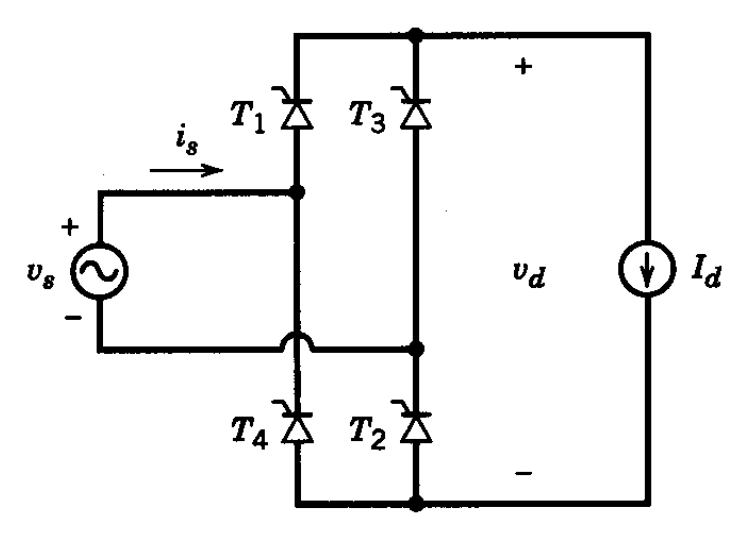
\includegraphics [width= 12 cm ]{singlephthyristor.png}
\caption{Single Phase Fully-Controlled Rectifier Structure}
\label{SingleThyristor}
\end{figure}
\end{center}

During the positive half cycle of the input voltage thyristors T1 and T2 conducts the current after they are fired. In the negative half cycle of the input voltage, the current commutates from thyristors T1 and T2 to thyristors T3 and T4. The zero crossings of the input voltage waveform should be detected to synchronize the firing times of thyristors. By controlling the firing angle of the thyristors, the average of the output voltage can be controlled.

There are basically two operation modes of this rectifier topology: rectification mode and inverter mode.
In rectification mode, the average output voltage and current of the rectifier topology is positive. In this mode, power flows from ac (input/grid) side to the dc (output/load) side of the rectifier.

In inverter mode of operation, the average output voltage becomes negative while the output current is still positive. Hence, the power flows from dc (output/load) side to ac (input/grid) side. In other words, the rectifier supplies back power to the grid. In order for this rectifier topology to operate in this mode, there should exist an active source element at the output/load side of the topology. 

Theoretical calculation for the average output voltage of the topology is given below:
\begin{equation}
    V_{avg} = \frac{2 \sqrt{2}}{\pi} V_{ph} \cos{\alpha} 
\end{equation}
A capacitor with large capacitance value can be connected in the load side of the rectifier in order to filter the output voltage, and reduce the output voltage ripple.

\subsubsection{Advantages}
\begin{itemize}
    \item The output voltage can be fully controlled by controlling the firing angles the thyristors.
    \item The structure of the topology is quite simple. It consists of only 4 thyristors.
    \item Its operation is also quite simple compared to three phase topologies and buck converter topology.
    \item It can be operated in four quadrant by connecting two Single Phase Thyristor Rectifier topologies back to back. When it is operated in its inverter mode, the rectifier can supply power back to the grid if an active source is available in the load side of the rectifier. In other words, the output voltage can become negative while the current is still positive.
    \item Driving the gates of the thyristors in this topology is relatively simple compared to three phase topologies.
    \item Relatively less number of components are required to construct the topology compared to three phase topologies. Only 4 thyristors and two gate drivers are required. Therefore, the topology is small in size.
\end{itemize}
\subsubsection{Disadvantages}
\begin{itemize}
    \item The output voltage ripple is quite high. The output voltage waveform follows the input voltage waveform. Hence, its ripple is equal to the input voltage ripple depending on the firing angle. In order to reduce the output voltage ripple, a large capacitor should be connected to the output of the rectifier.
    \item The harmonics in the input current are problematic in this topology. All odd harmonics exist in the input current waveform. This results in high THD value for the input current. In order to reduce the effects of those odd harmonics, a large source inductance should be added to the grid (input) side. However, the addition of the source side inductance effects the commutation time of the rectifier circuit. The commutation time increases with increasing source side inductance.
    \item In general, driving the gates of the thyristors is quite tedius and troublesome. A driver circuit is required to drive the gates of the thyristors. Also, gates should be fired at precisely correct angles in order to ensure the synchronous operation of the thyristors.
    \item The zero crossings of the input voltage waveform should be detected to synchronize the firing angles of the thyristors. 
\end{itemize}

\subsection{Three Phase Thyristor}
Second topology constructed with thyristors is three phase fully controlled rectifier. It is named as it is because with thyristors the output voltage can be controlled without having any dc-dc converter at the output. In the lectures, three phase thyristors are covered, operation philosophy, advantages and disadvantages with explanations can be followed below:
\subsubsection{Operation and Structure}
In the Figure \ref{fig:ThreeThyristor} below, the topology can be observed:

\begin{center}
\begin{figure}[H]
\centering
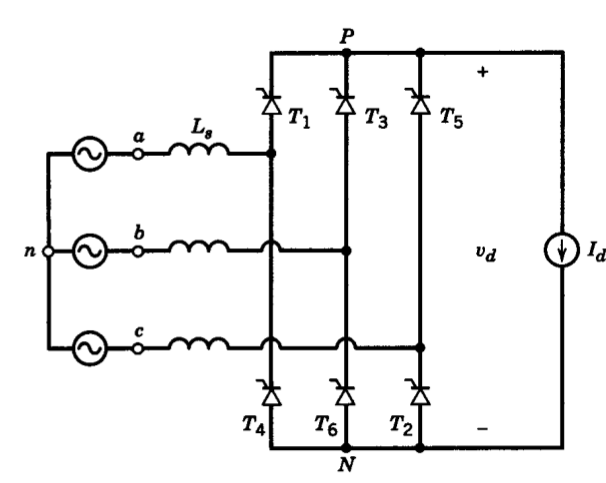
\includegraphics [width= 12 cm ]{ThreeThyristor.png}
\caption{Three Phase Fully-Controlled Rectifier Structure}
\label{fig:ThreeThyristor}
\end{figure}
\end{center}

In the three phase fully-controlled rectifier, six thyristors are used. Using gate signal generators, thyristors are fired in order to control output voltage. Theoretical calculation of output voltage is below:

\begin{equation}
    V_{avg} = \frac{3 \sqrt{2}}{\pi} V_{LL} \cos{\alpha} 
\end{equation}

\subsubsection{Advantages}
\begin{itemize}
    \item In this topology, output voltage can be controlled without any additional converter.
    \item Output ripple of this topology is respectively low. In order to decrease the ripple, a lower capacitor can be used in this topology.
    \item Third harmonic of input current is not observed in this topology. So, THD is respectively low.
    \item This topology can be used in inverter mode. Therefore, to obtain four quadrant operation, back to back three phase fully-controlled rectifiers can be utilized.
\end{itemize}

\subsubsection{Disadvantages}
\begin{itemize}
    \item This topology is built of six thyristors. Thyristors are expensive components comparing to the normal diodes. Therefore, this topology is more expensive than other options.
    \item In order to drive this rectifier, six different gate signals have to be used. This requires gate drivers and more components. It increases the cost, and it complicates the structure.
    \item Synchronization of gate drivers is hard. A zero crossing detector should be used in order to control it, it increases the cost and it makes the topology difficult.
\end{itemize}

\subsection{Three Phase Diode Rectifier with Buck Converter}
\subsubsection{Operation and Structure}
This topology consists of two parts. First part rectifies three phase ac grid voltage to low-ripple dc voltage. In the second part, we apply a buck converter and control our output voltage with duty cycle of switch. The first part of this topology is three phase diode rectifier. In the Figure \ref{fig:ThreeDiode} below the topology of three phase diode rectifier can be observed.

\begin{center}
\begin{figure}[H]
\centering
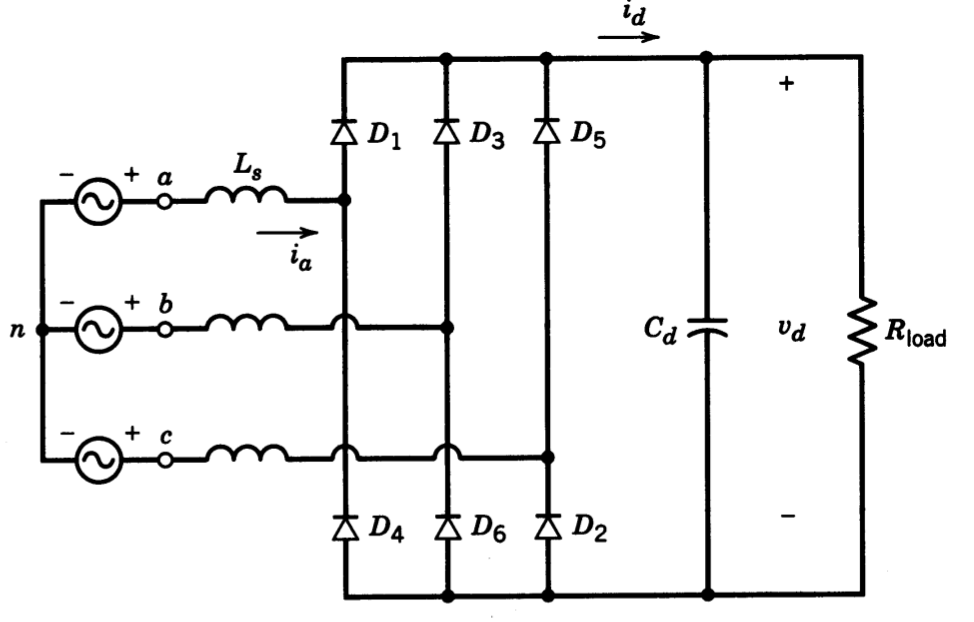
\includegraphics [width= 12 cm ]{threediode.png}
\caption{Three Phase Diode Rectifier Structure}
\label{fig:ThreeDiode}
\end{figure}
\end{center}

In three phase diode rectifier, one of upper diodes and one of bottom diodes conducts according to the phase voltage levels. In this topology we have no control of average output voltage. Below, theoretical output voltage can be observed.

\begin{equation}
    V_{avg} = \frac{3 \sqrt{2}}{\pi} V_{LL}
\end{equation}

In the Figure \ref{Buck} below, topology of step down converter can be examined.

\begin{center}
\begin{figure}[H]
\centering
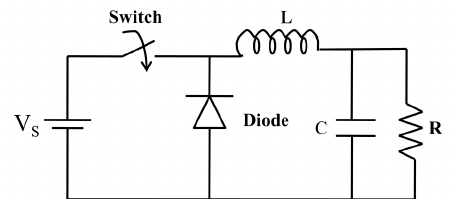
\includegraphics [width= 12 cm ]{buck.png}
\caption{Buck Converter Structure}
\label{Buck}
\end{figure}
\end{center}


Second part of this structure is buck converter. Buck converter basically step downs the input dc voltage to a desired level. In order to control output voltage, a MOSFET driven by a gate signal generator is used. Below, theoretical output voltage can be observed, D stands for duty cycle.

\begin{equation}
    V_{out} = DV_{in}
\end{equation}

Connecting diode rectifier and buck converter results in average voltage:
\begin{equation}
   V_{avg} = \frac{3 \sqrt{2}}{\pi} V_{LL} D
\end{equation}



\subsubsection{Advantages}
\begin{itemize}
    \item In this topology output voltage ripple is respectively low. 
    \item This topology requires only one gate signal which will be provided to drive buck converter. Thus, this is system is less complicated comparing to other topologies. Also, in this topology there is no need of synchronizing the signals.
    \item This topology consists of six diodes and a buck converter, this system is less expensive comparing to thyristor rectifiers.
    \item Since our motor is an LR load, we do not need to construct LC filter at the output of buck converter. This means this topology can be built easier.
\end{itemize}

\subsubsection{Disadvantages}
\begin{itemize}
    \item This topology does not support four quadrant operation. Diode rectifier can work in only one quadrant, so there is no way to obtain four quadrant.
    \item Theoretically, the expected efficiency is lower than thyristor cases because we use external diode in the buck converter.
\end{itemize}